\section{Filip Duda}
\label {flpdda}

Here's a picture of a mango (Picture \ref{fig:mng})

\begin{figure}[htbp]
    \centering
    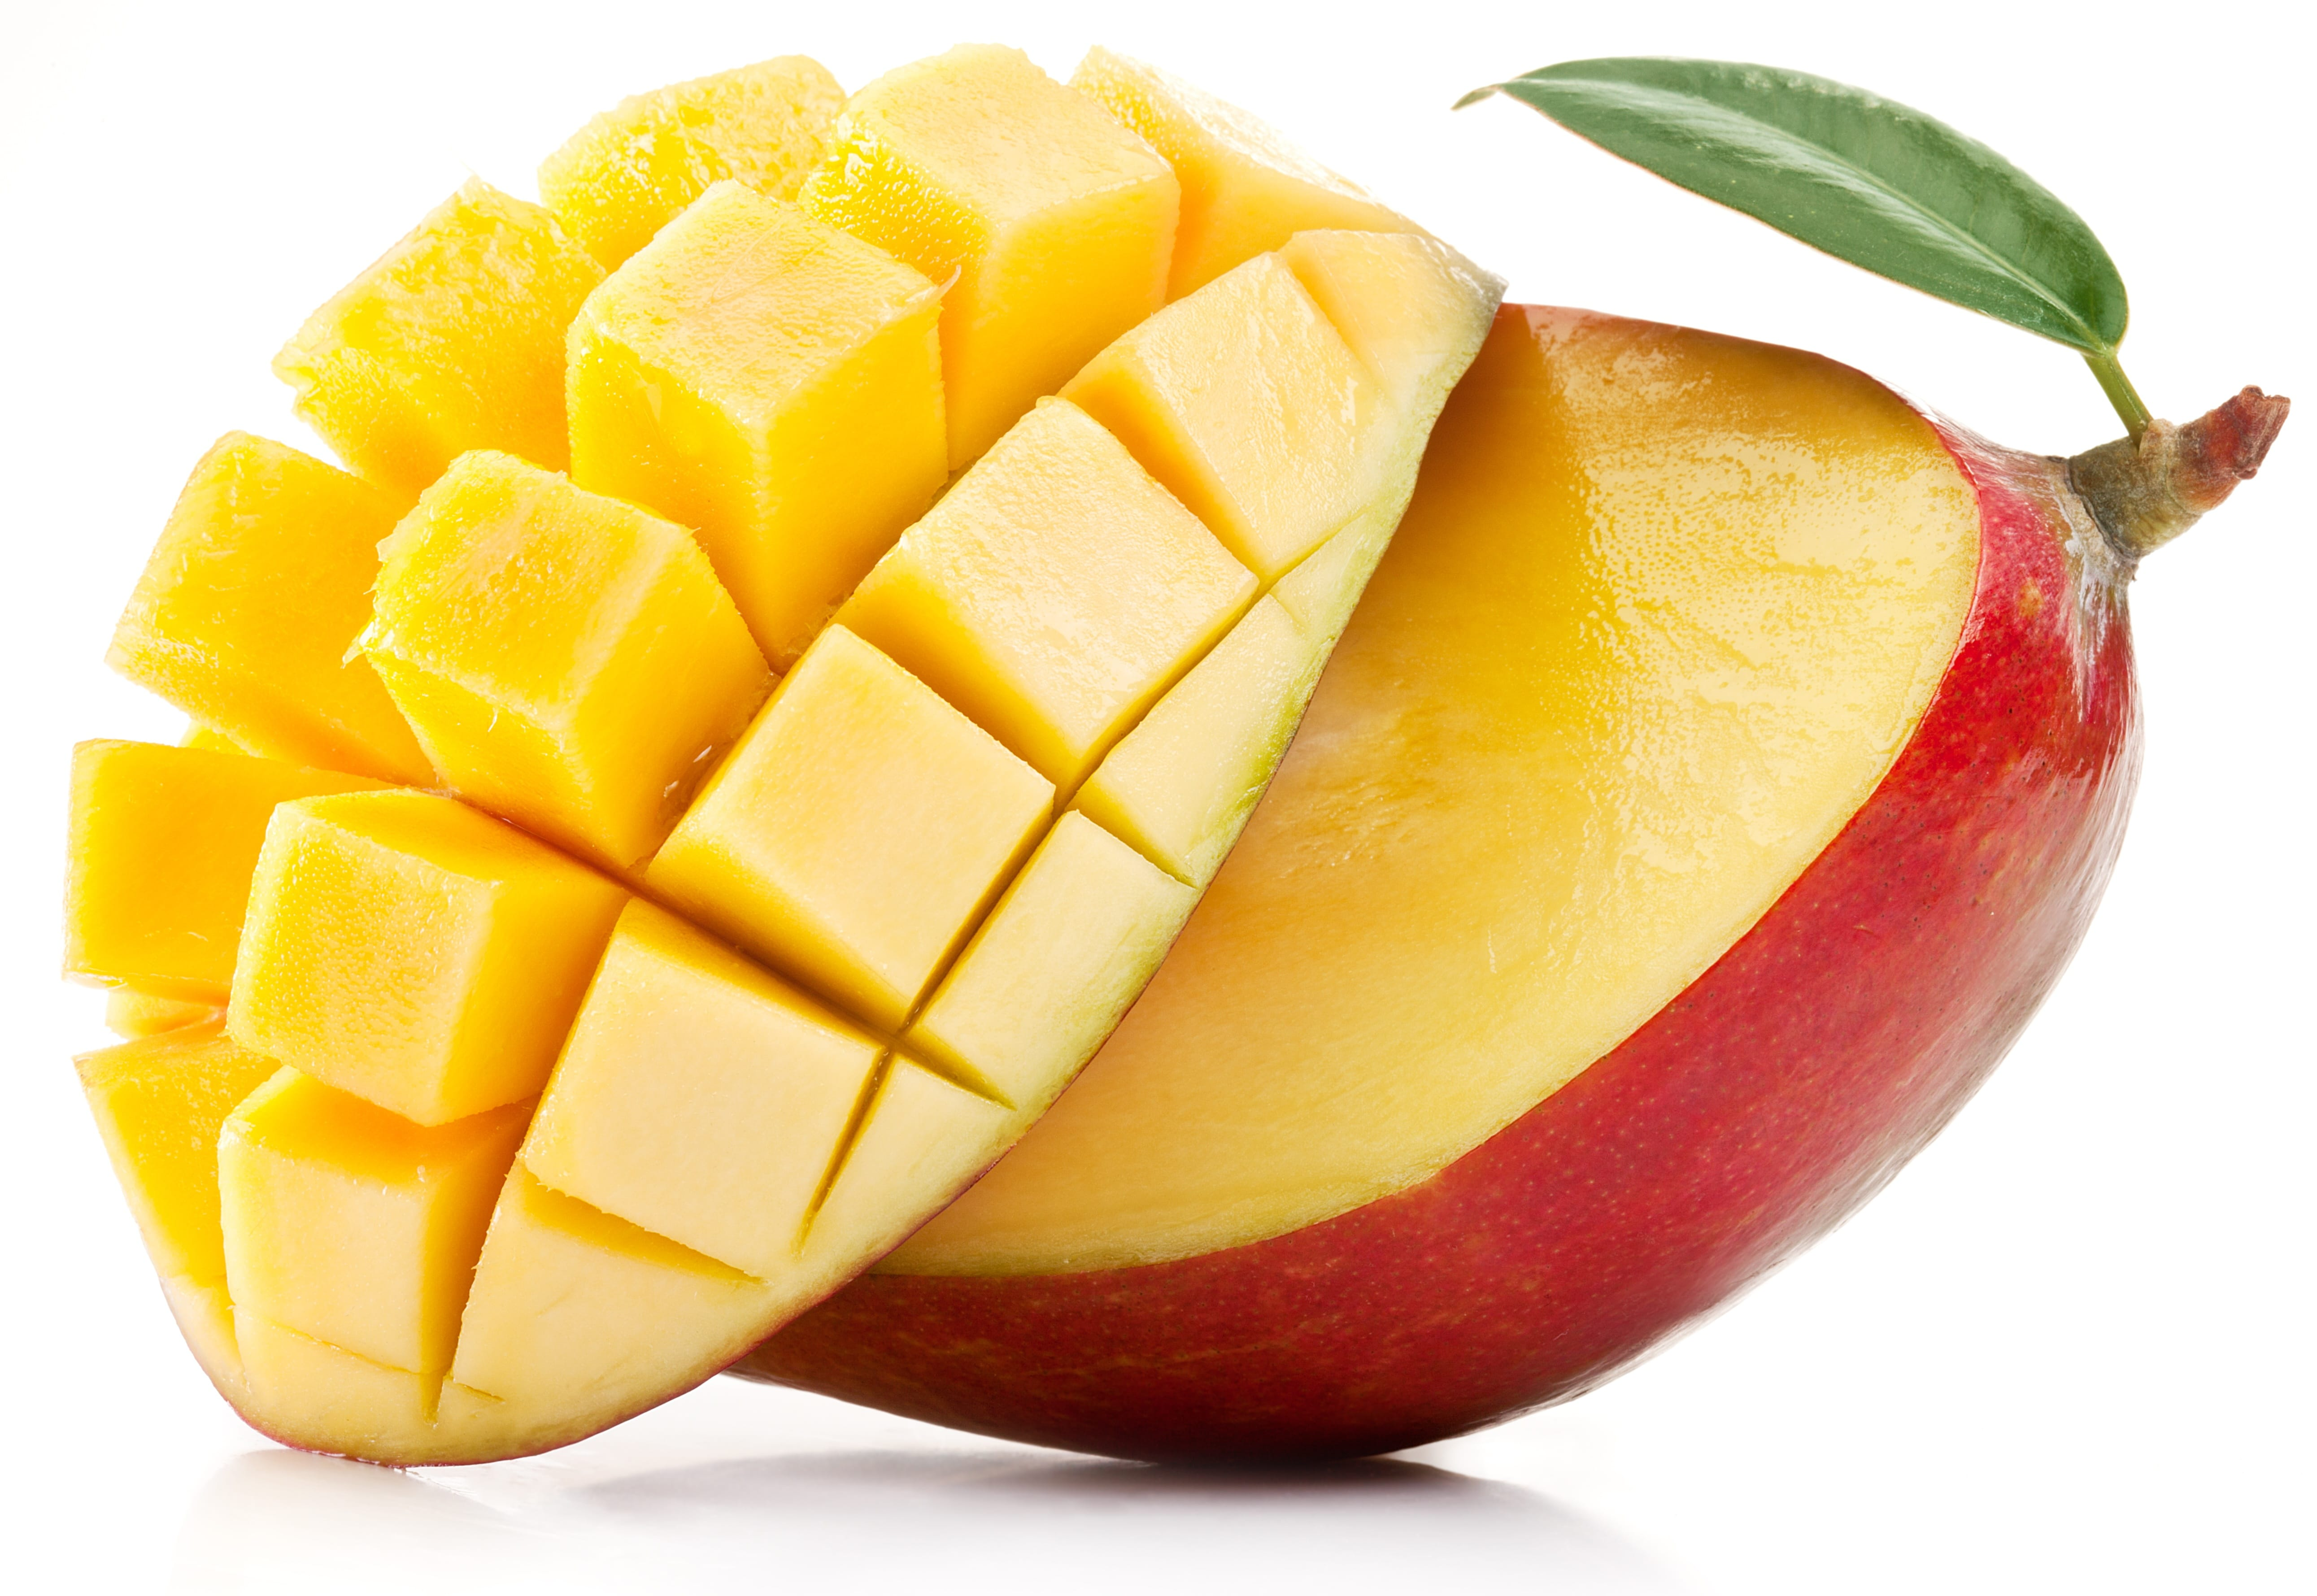
\includegraphics[width=0.7\textwidth]{Pictures/man-go.jpg}
    \caption{This is a mango.}
    \label{fig:mng}
\end{figure}
\begin{align*}
    Mango is native to India and Southeast Asia, and people have cultivated it for over 4,000 years. Hundreds of types of mango exist, each with its own characteristic taste, shape, size, and color.
    \par Mango trees grow to 30–40 metres (98–131 feet) tall, with a crown radius of 10–15 m (33–49 ft). The trees are long-lived, as some specimens still fruit after 300 years. The ripe fruit varies according to cultivar in size, shape, color, sweetness, and eating quality. Depending on the cultivar, fruits are variously yellow, orange, red, or green. The fruit has a single flat, oblong pit that can be fibrous or hairy on the surface and does not separate easily from the pulp. The fruits may be somewhat round, oval, or kidney-shaped, ranging from 5–25 centimetres (2–10 in) in length and from 140 grams (5 oz) to 2 kilograms (5 lb) in weight per individual fruit. The skin is leather-like, waxy, smooth, and fragrant.
\end{align*}

\newpage

Table ~\ref{mngtab} shows nutrition facts in a portion of mango.

\begin{table}[htbp]
\begin{tabular}{|lllll|}
\hline
\multicolumn{5}{|l|}{Nutrition facts per 165 grams of mango} \\ \hline
\multicolumn{4}{|l|}{Calories}           & 99 kcal           \\ \hline
\multicolumn{4}{|l|}{Protein}            & 1.4 grams         \\ \hline
\multicolumn{4}{|l|}{Carbs}              & 24.7 grams        \\ \hline
\multicolumn{4}{|l|}{Fat}                & 0.6 grams         \\ \hline
\multicolumn{4}{|l|}{Fiber}              & 2.6 grams         \\ \hline
\multicolumn{4}{|l|}{Sugar}              & 22.5 grams        \\ \hline
\multicolumn{4}{|l|}{Vitamin C}          & 67\%*             \\ \hline
\multicolumn{4}{|l|}{Vitamin B6}         & 12\%*             \\ \hline
\multicolumn{4}{|l|}{Vitamin A}          & 10\%*             \\ \hline
\multicolumn{4}{|l|}{Vitamin E}          & 10\%*             \\ \hline
\end{tabular}
\label{mngtab}
\caption{*percent of daily value}
\end{table}

Mango has many different health benefits. Some of them are:
\begin{itemize}[]
    \item[-] Improves cell function
    \item[-] Aids fluid balance
    \item[-] Protects against cell damage
    \item[-] Provides anti-inflammatory benefits
    \item[-] Boosts Vitamin A
    \label{hlthbf}
\end{itemize}

Mango also contains other nutrients that may also support immunity, including:
\begin{enumerate}
    \item copper
    \item folate
    \item vitamin E
    \item several B vitamins
\end{enumerate}

In order to stay healthy, it's important to know your BMI. Here's an equation to help you determine your BMI: \[BMI = \frac{mass[kg]}{height^2[m]}\]


